\section{Improvement of ATHLET-NuT communication}
\subsection{Overview of Jacobian matrix compression algorithm}


%%%%%%%%%%%%%%%%%%%%%%%%%%%%%%%%%%%%%%%%%%%%%%%%%%%%%%%%%%
\begin{frame}[t]{Jacobian Matrix Approximation}
    \spc
    \justifying
    %\small
    
    In the general case, \textbf{finite difference} method can be used to compute a \textbf{Jacobian} matrix \textbf{approximation} in the following way:
    
    \begin{equation} \label{eq:matrix-compression-1}
	    \frac{1}{\epsilon} (F(y + \epsilon e_{k}) - F(y)) \approx J(y) e_{k}, \: \: \: 1 \leq k \leq N
    \end{equation}

    where $F : \mathbb{R}^{N} \rightarrow \mathbb{R}^{N}$  is a non-linear function, $e_{k} \in \mathbb{R}^{N}$ is the k\textit{th}  \textbf{coordinate} unit \textbf{vector}, $\epsilon$ is a small step size.\\
    
    \begin{block}{Drawbacks:}
        \begin{itemize}
            \item Matrix sparsity is not exploited
            \item Requires $N$ function evaluations
        \end{itemize}
    \end{block}
    
\end{frame}

\ifSpeech
%%%%%%%%%%%%%%%%%%%%%%%%%%%%%%%%%%%%%%%%%%%%%%%%%%%%%%%%%%
\begin{frame}[t]{Compression, Matrix Partitioning}
    \justifying
    \small
    
    Compression is based on the notion of \textbf{structurally orthogonal} columns\\ 
    i.e. \underline{columns which do not share any non-zero entry in a common row}.
    
    \spc
        
    \textbf{Example:}
        \begin{itemize}
            \item Instead of using 5 coordinate unit vectors $e_{k}$, where $1 \leq k \leq 5 $  
            \item The same Jacobian can be approximated with \textbf{3 seed vectors} $d$: $d_{1} = [1,0,1,0,0]^{T}$, $d_{2} = [0,1,0,0,0]^{T}$, $d_{3} = [0,0,1,0,1]^{T}$
    \end{itemize}

        
    \begin{figure}[htpb]
        \centering
        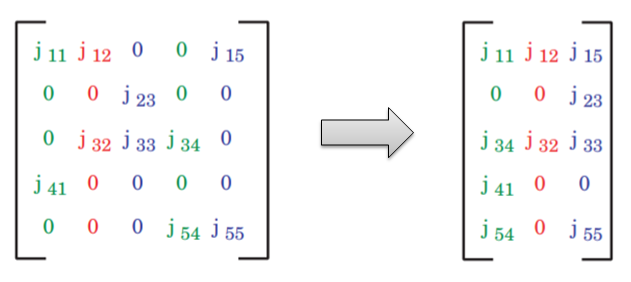
\includegraphics[width=0.50\textwidth]{figures/chapter-3/matrix-compression-example.png}
        \caption{An example of matrix coloring and compression \cite{gebremedhin2005color}}
        \label{fig:example-of-matrix-compression}
    \end{figure}
    

\end{frame}
\fi

%%%%%%%%%%%%%%%%%%%%%%%%%%%%%%%%%%%%%%%%%%%%%%%%%%%%%%%%%%
\begin{frame}[t]{Seeding, Partitioning, Compression}
    \justifying
    \small
    
    \begin{itemize}
        \item Seeding/Partitioning is based on \textbf{structurally orthogonal} columns i.e. columns which do not share any non-zero entry in a common row
    
        \item \textbf{efficiency} \textbf{requires} partitioning into \textbf{the fewest amount of} groups, \textbf{colors}, because evaluation of $F(y + \delta)$ is expensive
    \end{itemize}

    \begin{equation}
	    \frac{1}{\epsilon} (F(y + \epsilon d_{i}) - F(y)) \approx J(y) d_{i}, \: \: \: 1 \leq i \leq c << N
    \end{equation}
    
    \begin{figure}[htpb]
    \centering
    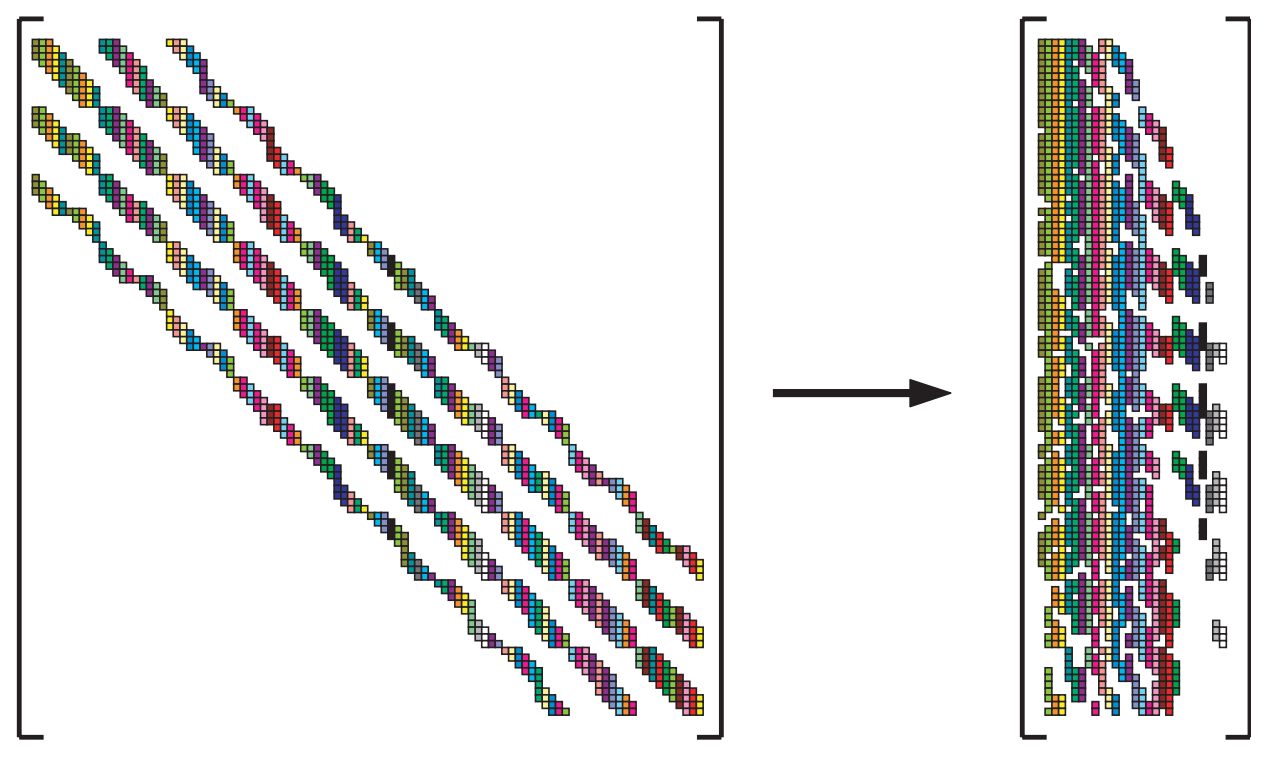
\includegraphics[width=0.5\textwidth]{figures/matrix-compression.png}
    \caption{An example of Jacobian matrix partitioning     \cite{gebremedhin2005color}}
    \end{figure}

\end{frame}


%%%%%%%%%%%%%%%%%%%%%%%%%%%%%%%%%%%%%%%%%%%%%%%%%%%%%%%%%%
\begin{frame}[t]{Arisen Problem due to ATHLET-NuT Design}
    \justifying
    \footnotesize

        \begin{itemize}
            \item Column vector \textbf{length} of the compressed Jacobian form is gradually \textbf{decreasing}
            
            \item Column length \textbf{distribution defines} the \textbf{communication pattern} between ATHLET and NuT
            
            \item Each \textbf{column transfer} is a service and, thus, it goes through \textbf{synchronous 3-way handshake} communication
            
        \end{itemize}


    \begin{columns}
    \column{0.7\textwidth}
        \begin{figure}[t]
            \centering
            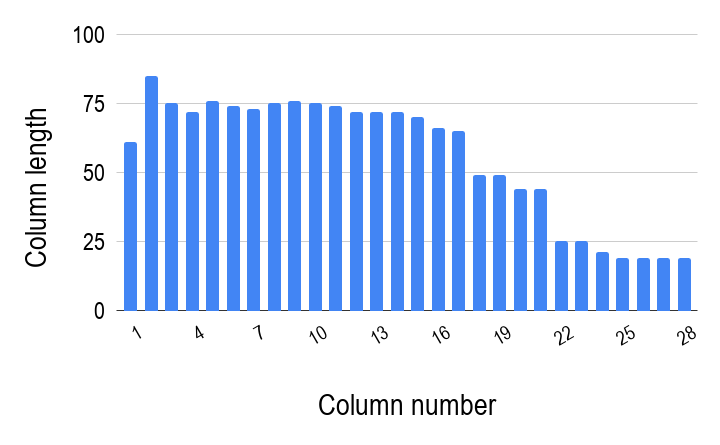
\includegraphics[width=0.9\textwidth]{figures/matrix-compression-2.png}
        \end{figure}
    \column{0.3\textwidth}
        \begin{figure}[t]
            \centering
            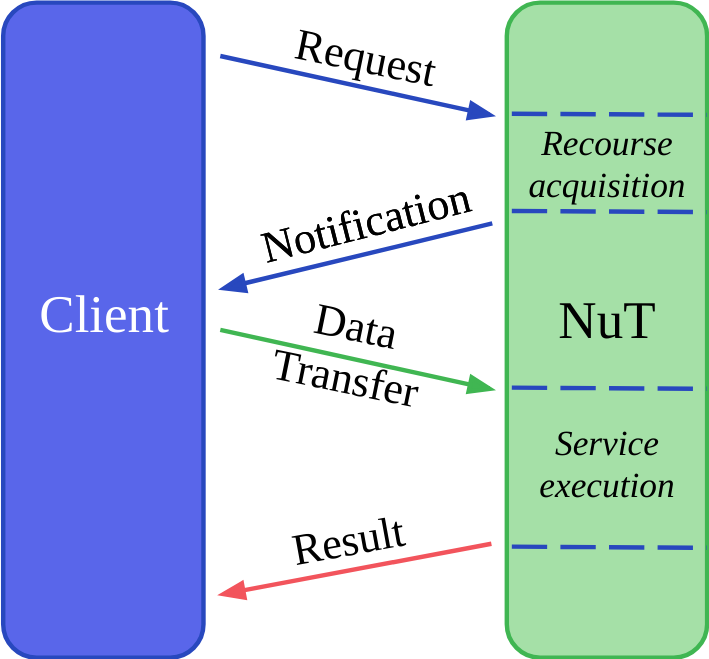
\includegraphics[width=0.9\textwidth]{figures/presentation-figures/handshake.png}
        \end{figure}
    \end{columns}

\end{frame}